\section{Assignment 2}
In this assignment we study the MCM system of equations, which models the interaction between three species of cells,
tumor-, healthy- and effector cells. The corresponding system of equations is given by
\begin{align*}
    T^{\prime} & =r_1 T\left(1-\frac{T}{k_1}\right)-a_{12} T H-a_{13} T E, \\
    H^{\prime} & =r_2 H\left(1-\frac{H}{k_2}\right)-a_{21} T H, \\
    E^{\prime} & =\frac{r_3 T E}{T+k_3}-a_{31} T E-d_3 E ,
\end{align*}
and its dimensionless form
\begin{align*}
    & x_1^{\prime}=x_1\left(1-x_1\right)-p_1 x_1 x_2-p_2 x_1 x_3, \\
    & x_2^{\prime}=p_3 x_2\left(1-x_2\right)-p_4 x_1 x_2, \\
    & x_3^{\prime}=\frac{p_5 x_1 x_3}{x_1+p_6}-p_7 x_1 x_3-p_8 x_3 .
\end{align*}

The parameters $p_i$ are specified in Table \ref{tab:mcm_parameters}
\begin{table}[H]
    \centering
    \begin{tabular}{|c|c|c|c|}
        \hline
        Parameter   & Definition                & description           & Value \\
        \hline
        $p_1$       & $\frac{a_{12}k_2}{r_1}$     & T->H competition      & 0.5 \\
        $p_2$       & $\frac{a_{31}k_1}{r_1}$     & E->T killing          & 2.5 \\
        $p_3$       & $\frac{r_2}{r_1}      $     & H-T growth ratio      & 0.6 \\
        $p_4$       & $\frac{a_{21}k_1}{r_1}$     & T->H inactivation     & 1.5 \\
        $p_5$       & $\frac{r_3k_2}{r_1}   $     & T->E stimulation      & 4.5 \\
        $p_6$       & $\frac{k_3}{k_1}      $     & E-T capacity ratio    & 1.0 \\
        $p_7$       & $\frac{a_{31}k_3}{r_1}$     & T->E inactivation     & 0.2 \\
        $p_8$       & $\frac{d_3}{r_1}      $     & E natural death       & 0.5 \\
        \hline
    \end{tabular}
    \caption{Parameters of the dimensionless system}
    \label{tab:mcm_parameters}
\end{table}

The goal of this assignment is to study the dynamics of this system as the parameter $p_1$ is varied.
We aim to find the stationary points, bifurcations and (stable) limit cycles of the system, and study their stability.

Additionally, we aim to find the period doubling bifurcations of the limit cycles, and study the stability of the resulting
period-doubled limit cycles. Eventually, we aim to determine the period doubling route to chaos.

\subsection{Stationary points}
Table \ref{tab:mcm_stationary_points} shows the stationary points of the system. 
\begin{table}[H]
	\begin{center}
		\begin{tabular}{|c|c|c|c|c|}
			\hline
			\textbf{index} & $\mathbf{x_1}$ & $\mathbf{x_2}$ & $\mathbf{x_3}$ & \textbf{stability} \\
			\hline
			1 & -2.00 & 6.00 & 0.00 & Unstable \\
			2 & 0.00 & 0.00 & 0.00 & Unstable \\
			3 & 0.00 & 1.00 & 0.00 & Unstable \\
			4 & 1.33$\times 10^{-1}$ & 0.00 & 3.47$\times 10^{-1}$ & Unstable \\
			5 & 1.33$\times 10^{-1}$ & 6.69$\times 10^{-1}$ & 2.13$\times 10^{-1}$ & Stable \\
			6 & 1.00 & 0.00 & 0.00 & Unstable \\
			7 & 1.89$\times 10^{1}$ & -4.62$\times 10^{1}$ & 2.09 & Unstable \\
			8 & 1.89$\times 10^{1}$ & 0.00 & -7.15 & Stable \\
			\hline
		\end{tabular}
	\end{center}
	\caption{Stationary points of the MCM model.}
	\label{tab:mcm_stationary_points}
\end{table}

\subsection{Continuation of stationary points}
We observe two stable stationary points (indices 5 and 8). We continue these
points in the parameter $ p_1 \in [0.5, 1] $ and plot the continuation in Figure \ref{fig:mcm_continuation}.
\begin{figure}[H]
    \centering
    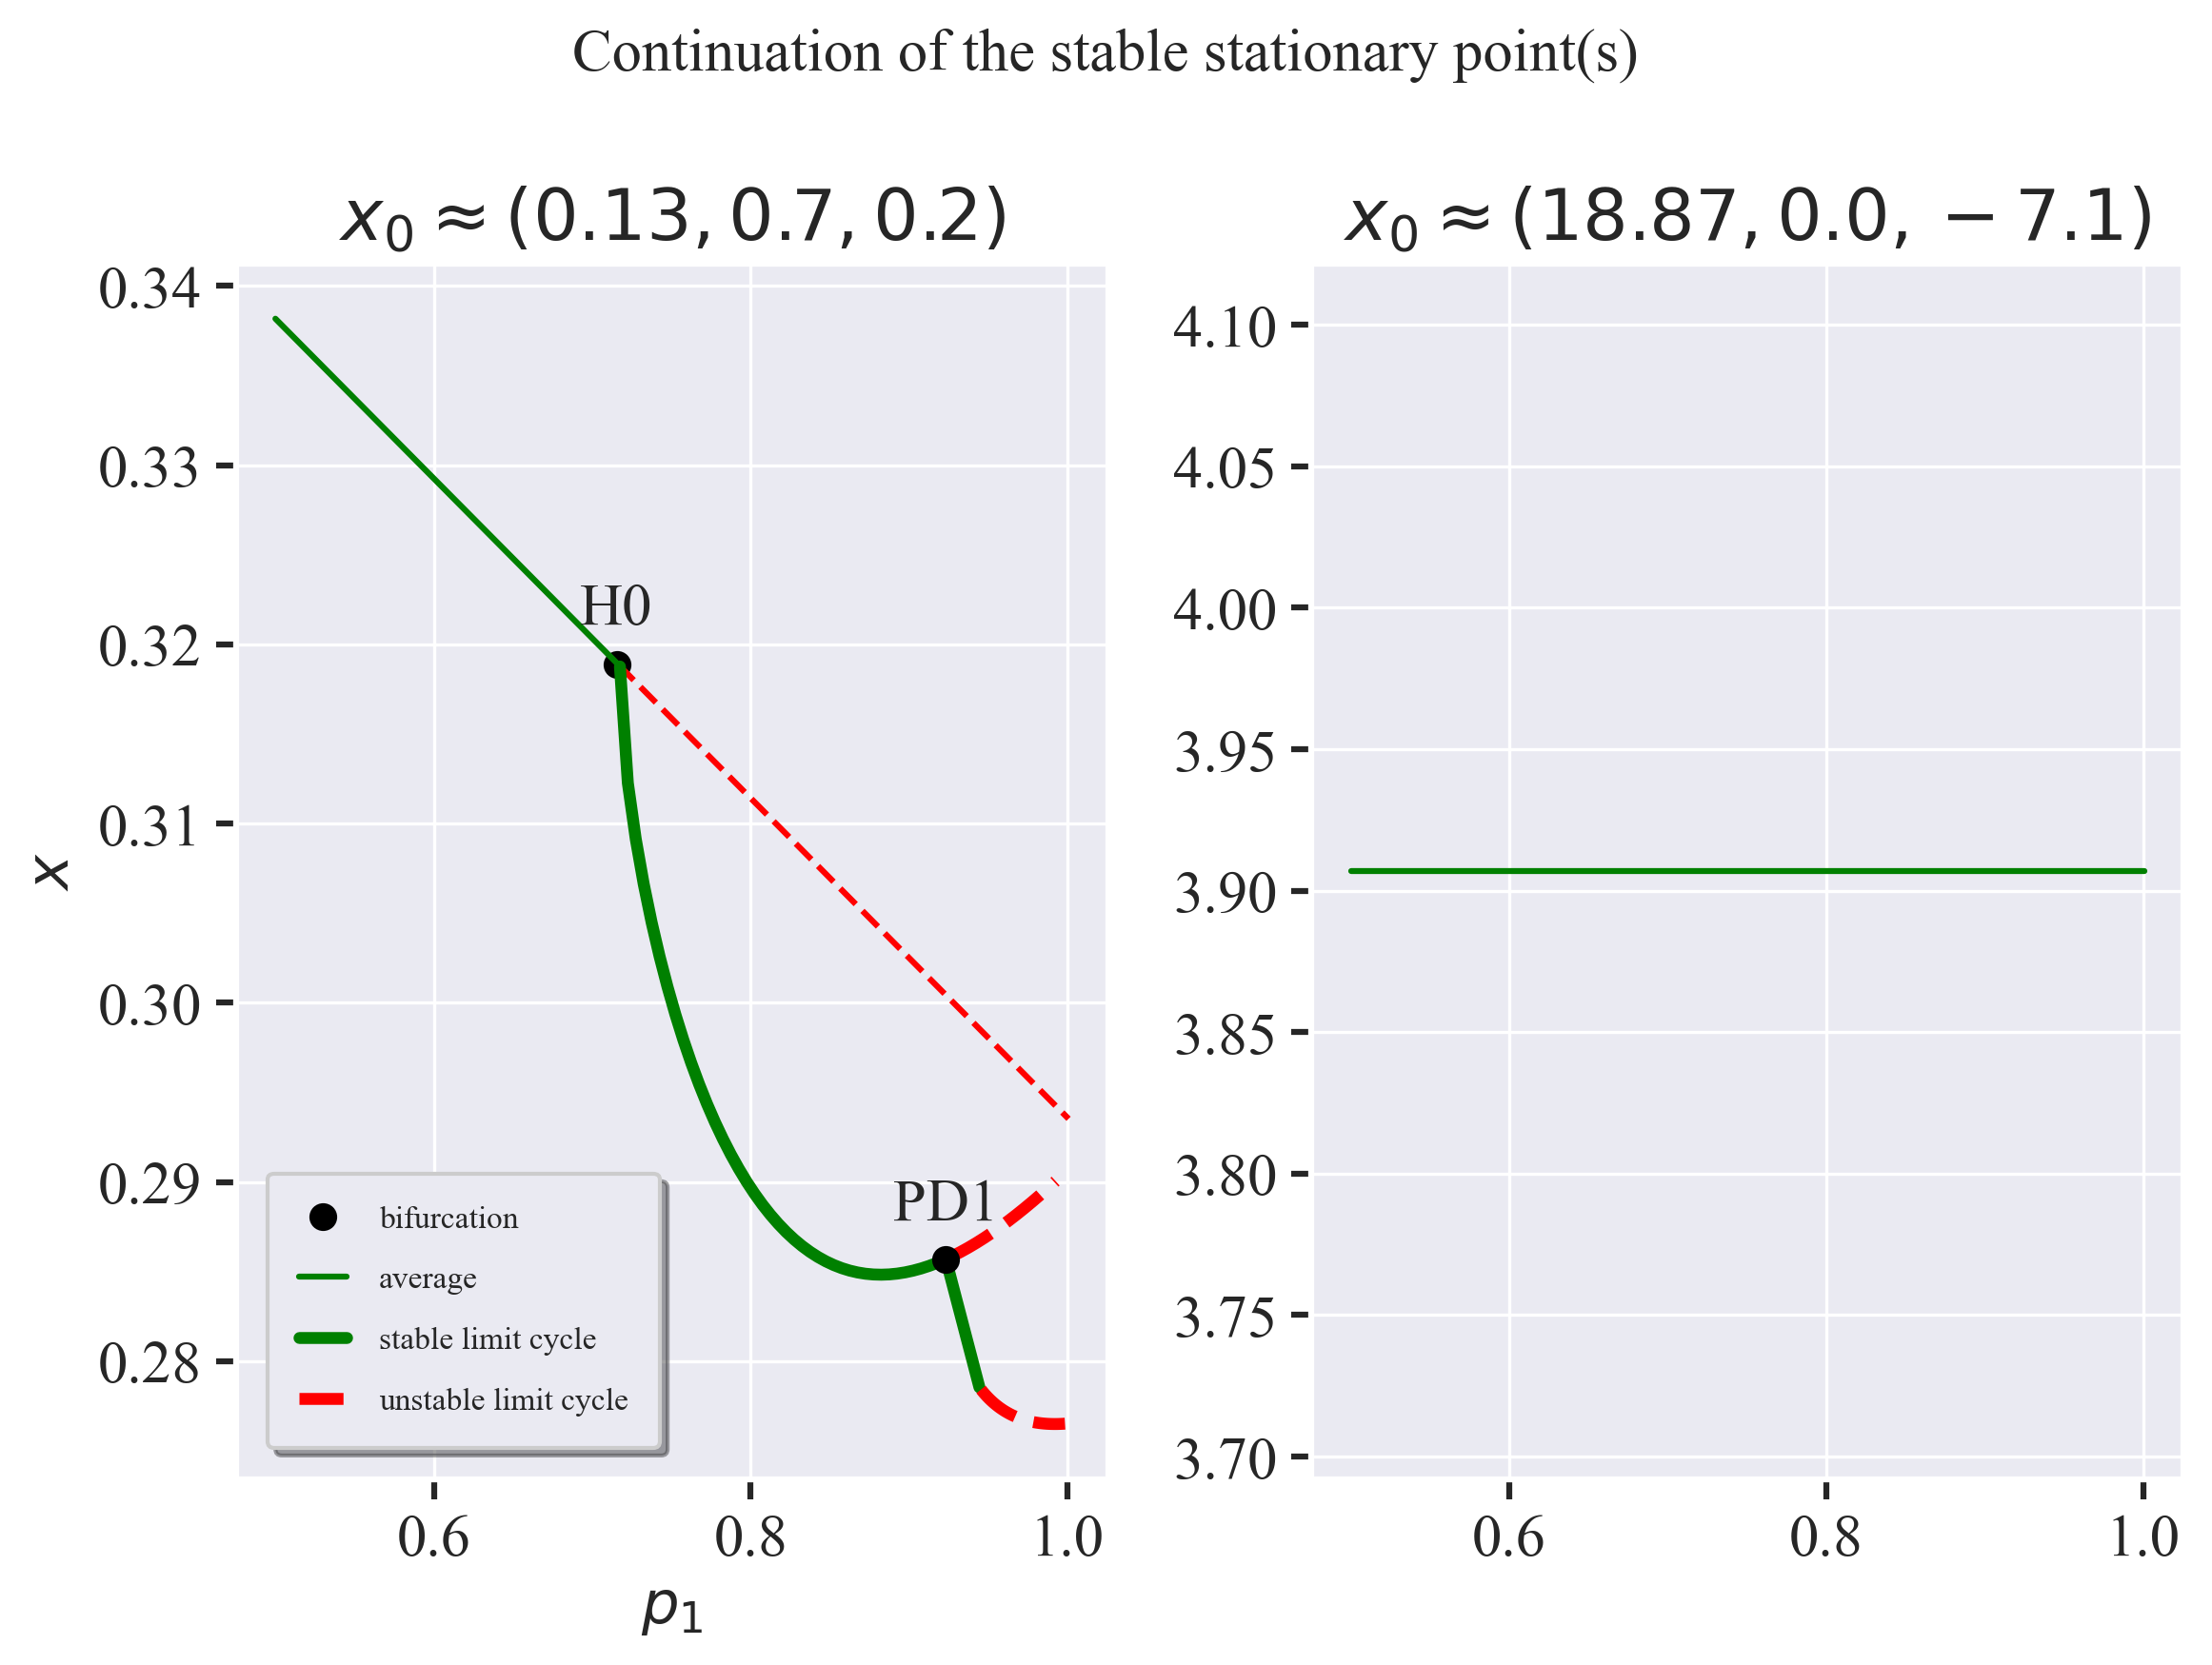
\includegraphics[width=0.8\textwidth]{figures/mcm_continuation.png}
    \caption{Continuation using the arc-length method of the stable stationary points in the parameter $p_1$,
    point 5 (left) and point 8 (right). The former encounters a bifurcation at $p_1 \approx 0.71$. From this 
    Hopf-bifurcation ($\textbf{H0}$) an unstable stationary solution and a stable limit cycle emerges. This limit cycle 
    then encounters a period doubling bifurcation at $p_1 \approx 0.923$ ($\textbf{PD1}$) and splits into a stable and unstable part.
    The stable part then encounters another period doubling bifurcation at $p_1 \approx 0.944$ ($\textbf{PD2}$) and splits again.
    The stable part of this limit cycle then encounters a third period doubling bifurcation at $p_1 \approx 0.949$ ($\textbf{PD3}$). However,
    the last bifurcation is not stable and the limit cycle seems to rejoin the original limit cycle.}
    \label{fig:mcm_continuation}
\end{figure}

The bifurcation that occurs during the continuation of point 5 in Figure \ref{fig:mcm_continuation} is given by
\begin{align*}
    \textbf{Bifurcation type} & : \text{Hopf} \\
    \textbf{Label} &: \text{H0} \\
    \textbf{Parameter} & : p_1 \\
    \textbf{Critical value} & : 0.71 \\
    \textbf{Eigenvalues} & : 0 \pm 0.36i, -0.53\\
    \mathbf{x}& : 0.13, 0.67, 0.16
\end{align*}
This bifurcation point was found by applying an indirect method based on the interpolation of test function values, adapted from 
Seydel's book (section 5.3.1). The particular test function used was the maximum of the real part of the eigenvalues of
the system Jacobian.

The bifurcation is a Hopf-bifurcation, as a complex pair of eigenvalues crosses the imaginary axis with non-zero velocity
That is to say, the eigenvalues of the system jacobian at the continuation step directly before and after the bifurcation are
\begin{align*}
    &\textbf{before: } &-1.4\times10^{-4} \pm 0.36i, -0.53,\\
    &\textbf{after: }  &1.38\times10^{-4} \pm 0.36i, -0.53	
\end{align*}
which shows the eigenvalues pass the imaginary axis with non-zero velocity.

From the (static) Hopf-bifurcation we determine the first dynamical solution using the method described in 
section 7.6.2 of Seydel's book. In other words we solve the following BVP 
\begin{align}
    \left(\begin{array}{l}
        \mathbf{x} \\
        T \\
        \lambda \\
        \mathbf{h}
        \end{array}\right)^{\prime}=\left(\begin{array}{c}
        T \mathbf{f}(\mathbf{x}, \lambda) \\
        0 \\
        0 \\
        T \mathbf{f}_{\mathbf{x}}(\mathbf{x}, \lambda) \mathbf{h}
        \end{array}\right), \quad\left(\begin{array}{c}
        \mathbf{x}(0)-\mathbf{x}(1) \\
        \mathbf{h}(0)-\mathbf{h}(1) \\
        \sum_i h_i \partial f_1 / \partial x_i \\
        h_1(0)-1
        \end{array}\right)=\mathbf{0},
\end{align}
using the shooting method in order to switch from the stationary solution to the limit cycle. In particular, we initialize the system 
to a point either on or close to the Hopf-bifurcation, because this point is close to the limit cycle. We then provide an initial guess for the 
period of the limit cycle, and solve the BVP using the shooting method. To do so, we make use of Scipy's \lstinline|integrate.solve_ivp| and \lstinline|optimize.fsolve| functions.
In short, the former allows us to integrate the system of ODEs, while the latter allows us to solve the BVP. 

Going into more detail, we use \lstinline|integrate.solve_ivp| 
\footnote{We use a maximum timestep of 0.001. I did not do initially and it gave the 
wrong results I discussed in my last submission. Same goes for the Floquet multipliers, for which
I used the same Scipy function. Fixing the max time step now gives the right values allowing me to find
the period doubling bifurcations.}
to integrate the system of ODEs over some period $T$ and then use the final values of the integration to calculate the residuals of the boundary conditions.
This defines an objective function that we want to minimize. We then use \lstinline|optimize.fsolve| to find the values of the initial conditions that make the residuals zero. \lstinline|optimize.fsolve| will 
effectively find the initial conditions that make the solution of the BVP a limit cycle.

The solution we obtain upon completing above process is
\begin{align*}
    \mathbf{x}^{(0)} & = (0.13, 0.67, 0.15)\\
    T^{(0)} &= 17.6\\
    p_1^{(0)} & = 0.72 \\
    \mathbf{h}^{(0)} &= (1.00, -1.40 , 0.00),
\end{align*}
from which we get a more accurate estimate for the period of the limit cycle.

\subsection{Continuation of limit cycle from Hopf-bifurcation}
We use the solution of the BVP from the previous section as an initial guess for the continuation of the limit cycle.
Following the method outlined in section 7.6.3 of Seydel's book, we continue the limit cycles from the dynamic Hopf-bifurcation 
point $(\mathbf{x}^{(0)}, T^{(0)}, p_1^{(0)}, \mathbf{h}^{(0)})$ in the parameter $p_1$ by repeatedly solving the boundary value problem 
(Seydel, Equation 7.6c, p. 306)
\begin{align}
    \left(\begin{array}{c}
        \mathbf{x} \\
        T \\
        \lambda
        \end{array}\right)^{\prime}=\left(\begin{array}{c}
        T \mathbf{f}(\mathbf{x}, \lambda) \\
        0 \\
        0
        \end{array}\right), \quad\left(\begin{array}{c}
        \mathbf{x}(0)-\mathbf{y}(1) \\
        f_j(\mathbf{y}(0), \lambda) \\
        p_1^{(k+1)}-p_1^{(k)} - \delta_p
        \end{array}\right)=\mathbf{0} ,
\label{eq:continuation_system}
\end{align}
where $\delta_p \approx = 0.005$ is a small value that determines the step size in the parameter $p_1$ and $j=1$ (phase condition).

The shooting method needs an initial guess, as it is really just a root finding algorithm. 
Therefore, each iteration starts with the solution of the previous iteration. 
Note that the first iteration starts with a small perturbation in the direction of $\mathbf{h}$ (Equation 7.24, Seydel)
\[
    \textbf{initial guess: }\mathbf{x}^{(k+1)} = 
    \begin{cases}
        \mathbf{x}^{(0)} + \delta_{\mathbf{h}}\mathbf{h}^{(0)}, & \text{if } k = 0, \\
        \mathbf{x}^{(k)}, & \text{otherwise},
    \end{cases}
    \quad T^{(k+1)} = T^{(k)}, \quad p_1^{(k+1)} = p_1^{(k)},
\]
for a suitably small parameter $\delta_{\mathbf{h}} \approx 0.01$. This results in a sequence of limit cycles starting from the Hopf point (k=0)
\[
    \textrm{cycle}^{(k)} = \left\{\mathbf{x}^{(k)}, T^{(k)}, p_1^{(k)} \right\}, \quad k = 0, 1, 2, \ldots
\]
which we integrate over their respective periods and plot in Figure \ref{fig:mcm_limit_cycle_continuation}.
\begin{figure}[H]
    \centering
    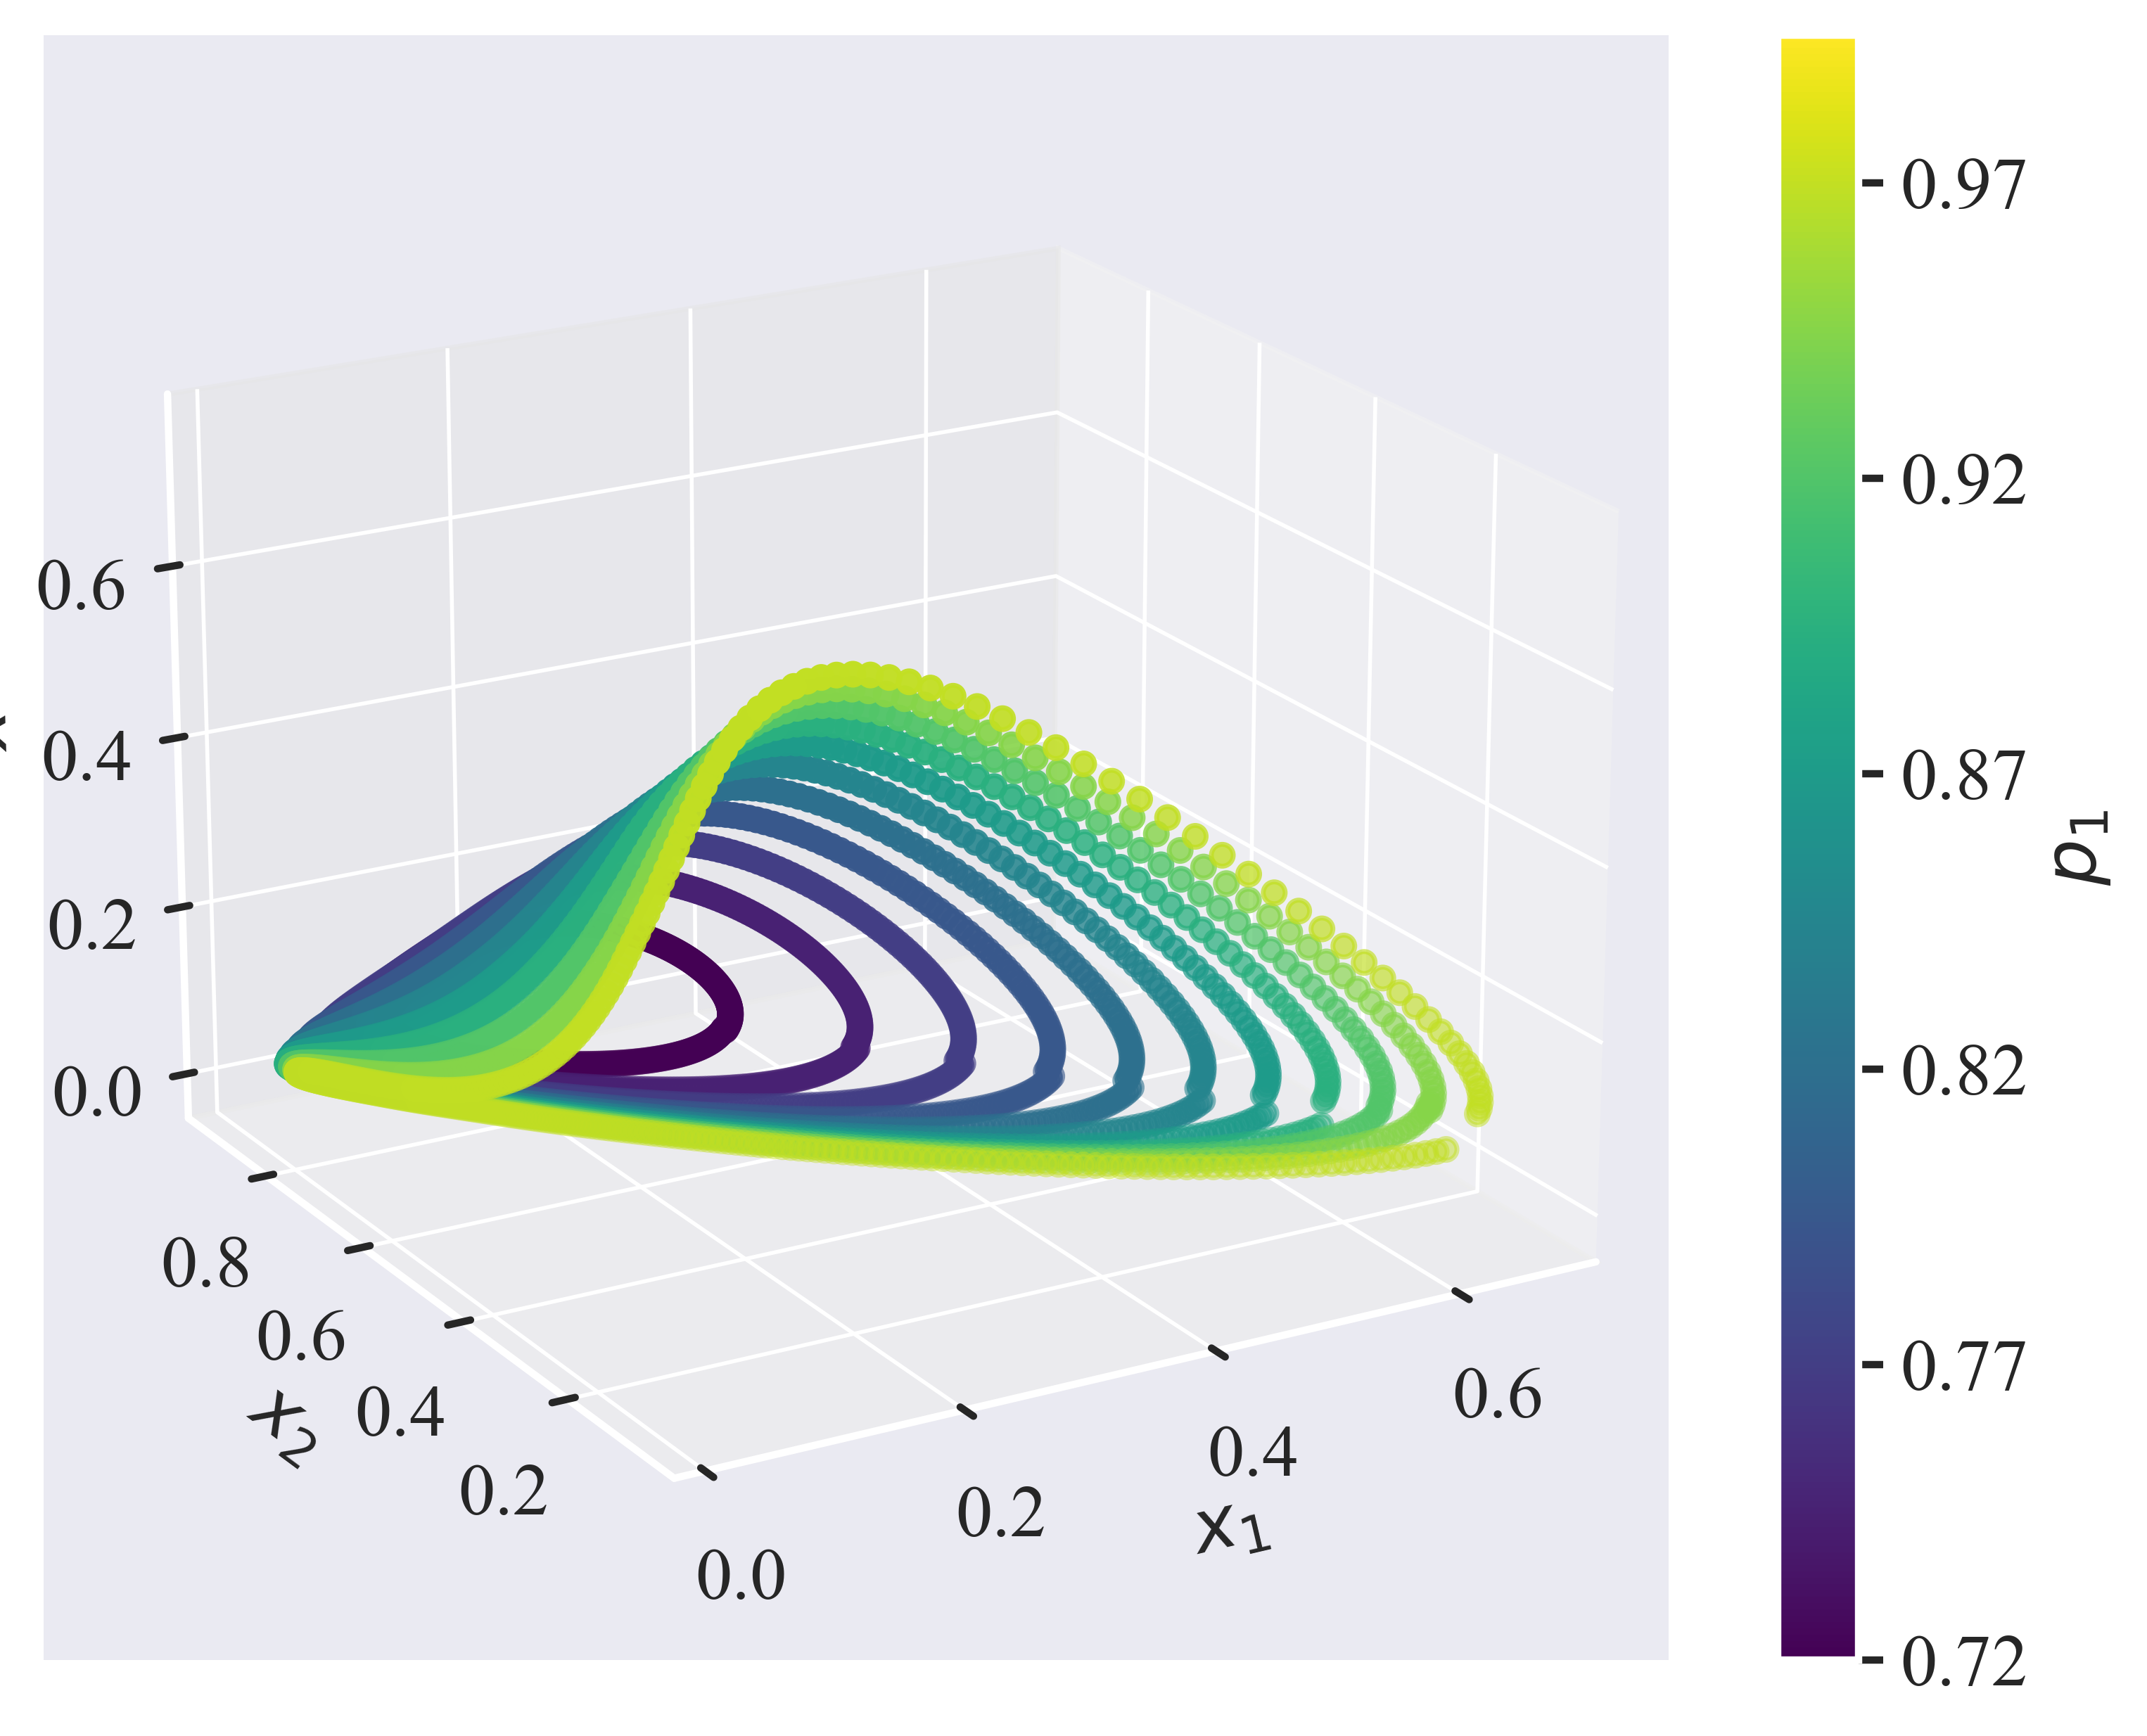
\includegraphics[width=0.7\textwidth]{figures/mcm_limit_cycles.png}
    \caption{Continuation of the limit cycle in the parameter $p_1$. The colors indicate the increase in $p_1$ from dark to light.}
    \label{fig:mcm_limit_cycle_continuation}
\end{figure}
The limit cycles in Figure \ref{fig:mcm_limit_cycle_continuation} are averaged both in time and in space to obtain the points in 
Figure \ref{fig:mcm_limit_cycle_continuation}; thick green line from \textbf{H0} to \textbf{PD1} and thick, dashed red line from 
\textbf{PD1} to the end of the graph.

For each limit cycle we calculate the monodromy matrix $M$ using Algorithm 7.12
from section 7.5.1 of Seydel. The eigenvalues of $M$ (Floquet multipliers) $\mu_j$ are then used to determine the stability of the limit cycle
(according to Summary 7.5, p. 315, Seydel).

The stability of the limit cycles obtained from this process is accordingly shown in Figure \ref{fig:mcm_continuation}, where 
the thick green- and thick, dashed red lines indicate stable and unstable limit cycles, respectively. 

\subsection{Period doubling bifurcations}
Period doubling bifurcations occur at those limit cycles where there is a $j$ for which $\mu_j = -1$.
Hence, we continue the limit cycle (and calculate the monodromy matrices) until we find a multiplier close to $-1$.\footnote{We use a tolerance of 0.01.}
We then use interpolation to find the exact value of $p_1$ at which the period doubling bifurcation occurs.
Doing this for the limit cycle we discussed in the previous section we find the
\textbf{first period doubling bifurcation: } 
\begin{align*}
    \textbf{Bifurcation type} & : \text{period doubling} \\
    \textbf{Label} &: \text{PD1} \\
    \textbf{Parameter} & : p_1 \\
    \textbf{Critical value} & : 0.923 \\
    \textbf{Floquet multipliers} & : -1.00, 0, 1.00 \leftarrow \text{note the -1} \\
    \mathbf{x}  & = (0.59, 0.17, 0.10) \\
    \textbf{Period} & : 31.55 \\
\end{align*}
Starting from this interpolated period doubling bifurcation point we 
apply the shooting method to solve the BVP in Equation 7.27 of Seydel's book. 
\begin{align}
    \left(\begin{array}{c}
        \mathbf{x} \\
        T \\
        \lambda \\
        \mathbf{h}
        \end{array}\right)^{\prime}=\left(\begin{array}{c}
        T \mathbf{f}(\mathbf{x}, \lambda) \\
        0 \\
        0 \\
        T \mathbf{f}_{\mathbf{x}}(\mathbf{x}, \lambda) \mathbf{h}
        \end{array}\right), \quad\left(\begin{array}{c}
        \mathbf{x}(0)-\mathbf{x}(1) \\
        p(\mathbf{x}(0), \lambda) \\
        \mathbf{h}(0)+\mathbf{h}(1) \\
        h_k(0)-1
        \end{array}\right)=\mathbf{0} .
\end{align}
This gives a point on the period doubled branch $(\mathbf{x}^{(0)}, T^{(0)}, p_1^{(0)}, \mathbf{h}^{(0)})$, 
which we can continue in the same way as we did in the previous section.
That is to say, we repeatedly apply the shooting method to BVP in Equation \ref{eq:continuation_system} 
The only differences being that we take slightly smaller steps $\delta_p = 0.001$, and 
we specify slightly different initial guesses for the continuation of the period-doubled limit cycle. Namely,
\begin{align*}
    \textbf{initial guess: }&\mathbf{x}^{(k+1)} = 
    \begin{cases}
        \mathbf{x}^{(0)} + \delta \mathbf{h}^{(0)}, & \text{if } k = 0, \\
        \mathbf{x}^{(k)}, & \text{otherwise},
    \end{cases} \\
    &T^{(k+1)} = 
    \begin{cases}
        2 T^{(0)}, & \text{if } k = 0, \\
        T^{(k)}, & \text{otherwise}, 
    \end{cases}\\
    &p_1^{(k+1)} = p_1^{(k)}.
\end{align*}
This results in Figure \ref{fig:mcm_period_doubled_branch} where we plot the period-doubled limit cycles in the parameter $p_1$.
\begin{figure}
    \centering
    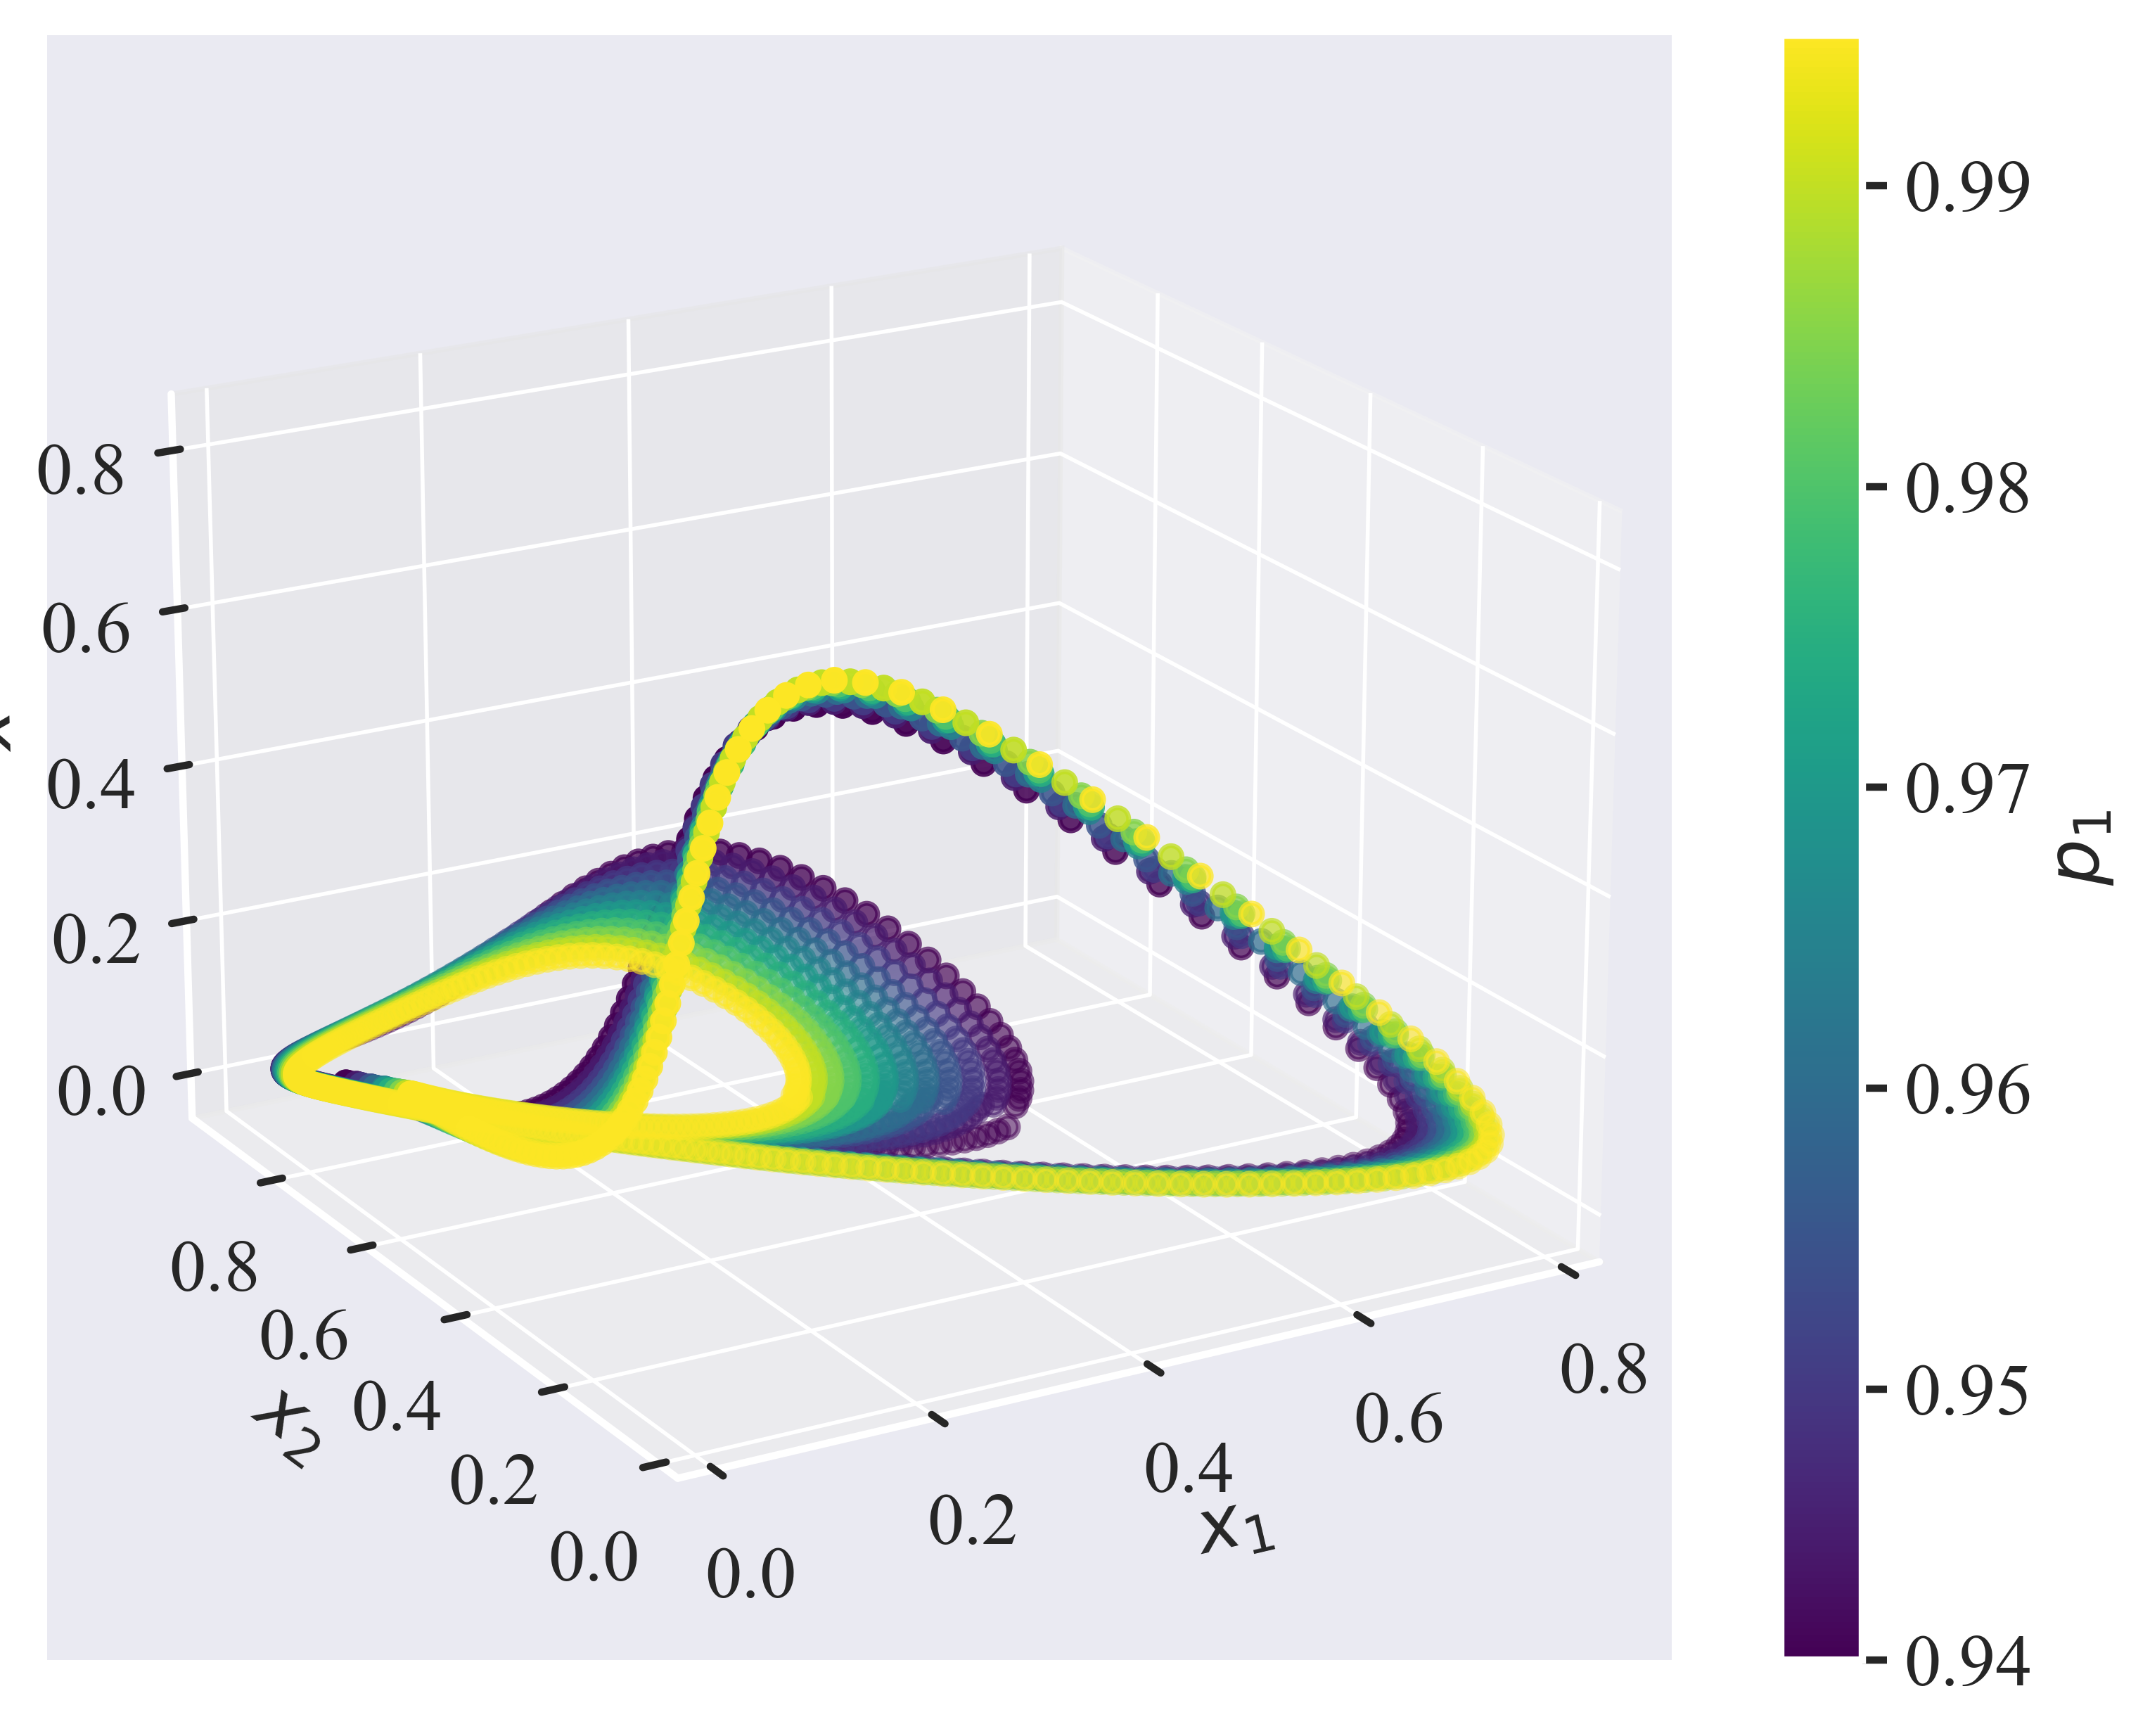
\includegraphics[width=0.7\textwidth]{figures/mcm_first_pdouble.png}
    \caption{Similar to Figure \ref{fig:mcm_limit_cycle_continuation}, but now showing the period-doubled limit cycles. Note the double loop 
    in the limit cycle.}
    \label{fig:mcm_period_doubled_branch}
\end{figure}

By again calculating the monodromy matrix and corresponding Floquet multipliers for every cycle, we find the second period-doubling bifurcation
\begin{align*}
    \textbf{Bifurcation type} & : \text{period doubling} \\
    \textbf{Label} &: \text{PD2} \\
    \textbf{Parameter} & : p_1 \\
    \textbf{Critical value} & : 0.944 \\
    \textbf{Floquet multipliers} & : -1.00, 0, 1.00 \\
    \mathbf{x}  & = (0.43, 0.28, 0.12) \\
    \textbf{Period} & : 64.92 \\
\end{align*}

We can continue the steps outlined above to find more period-doubling bifurcations. 
% This results in Figure \ref{fig:mcm_period_doubled_branch_2}
% \begin{figure}[H]
%     \centering
%     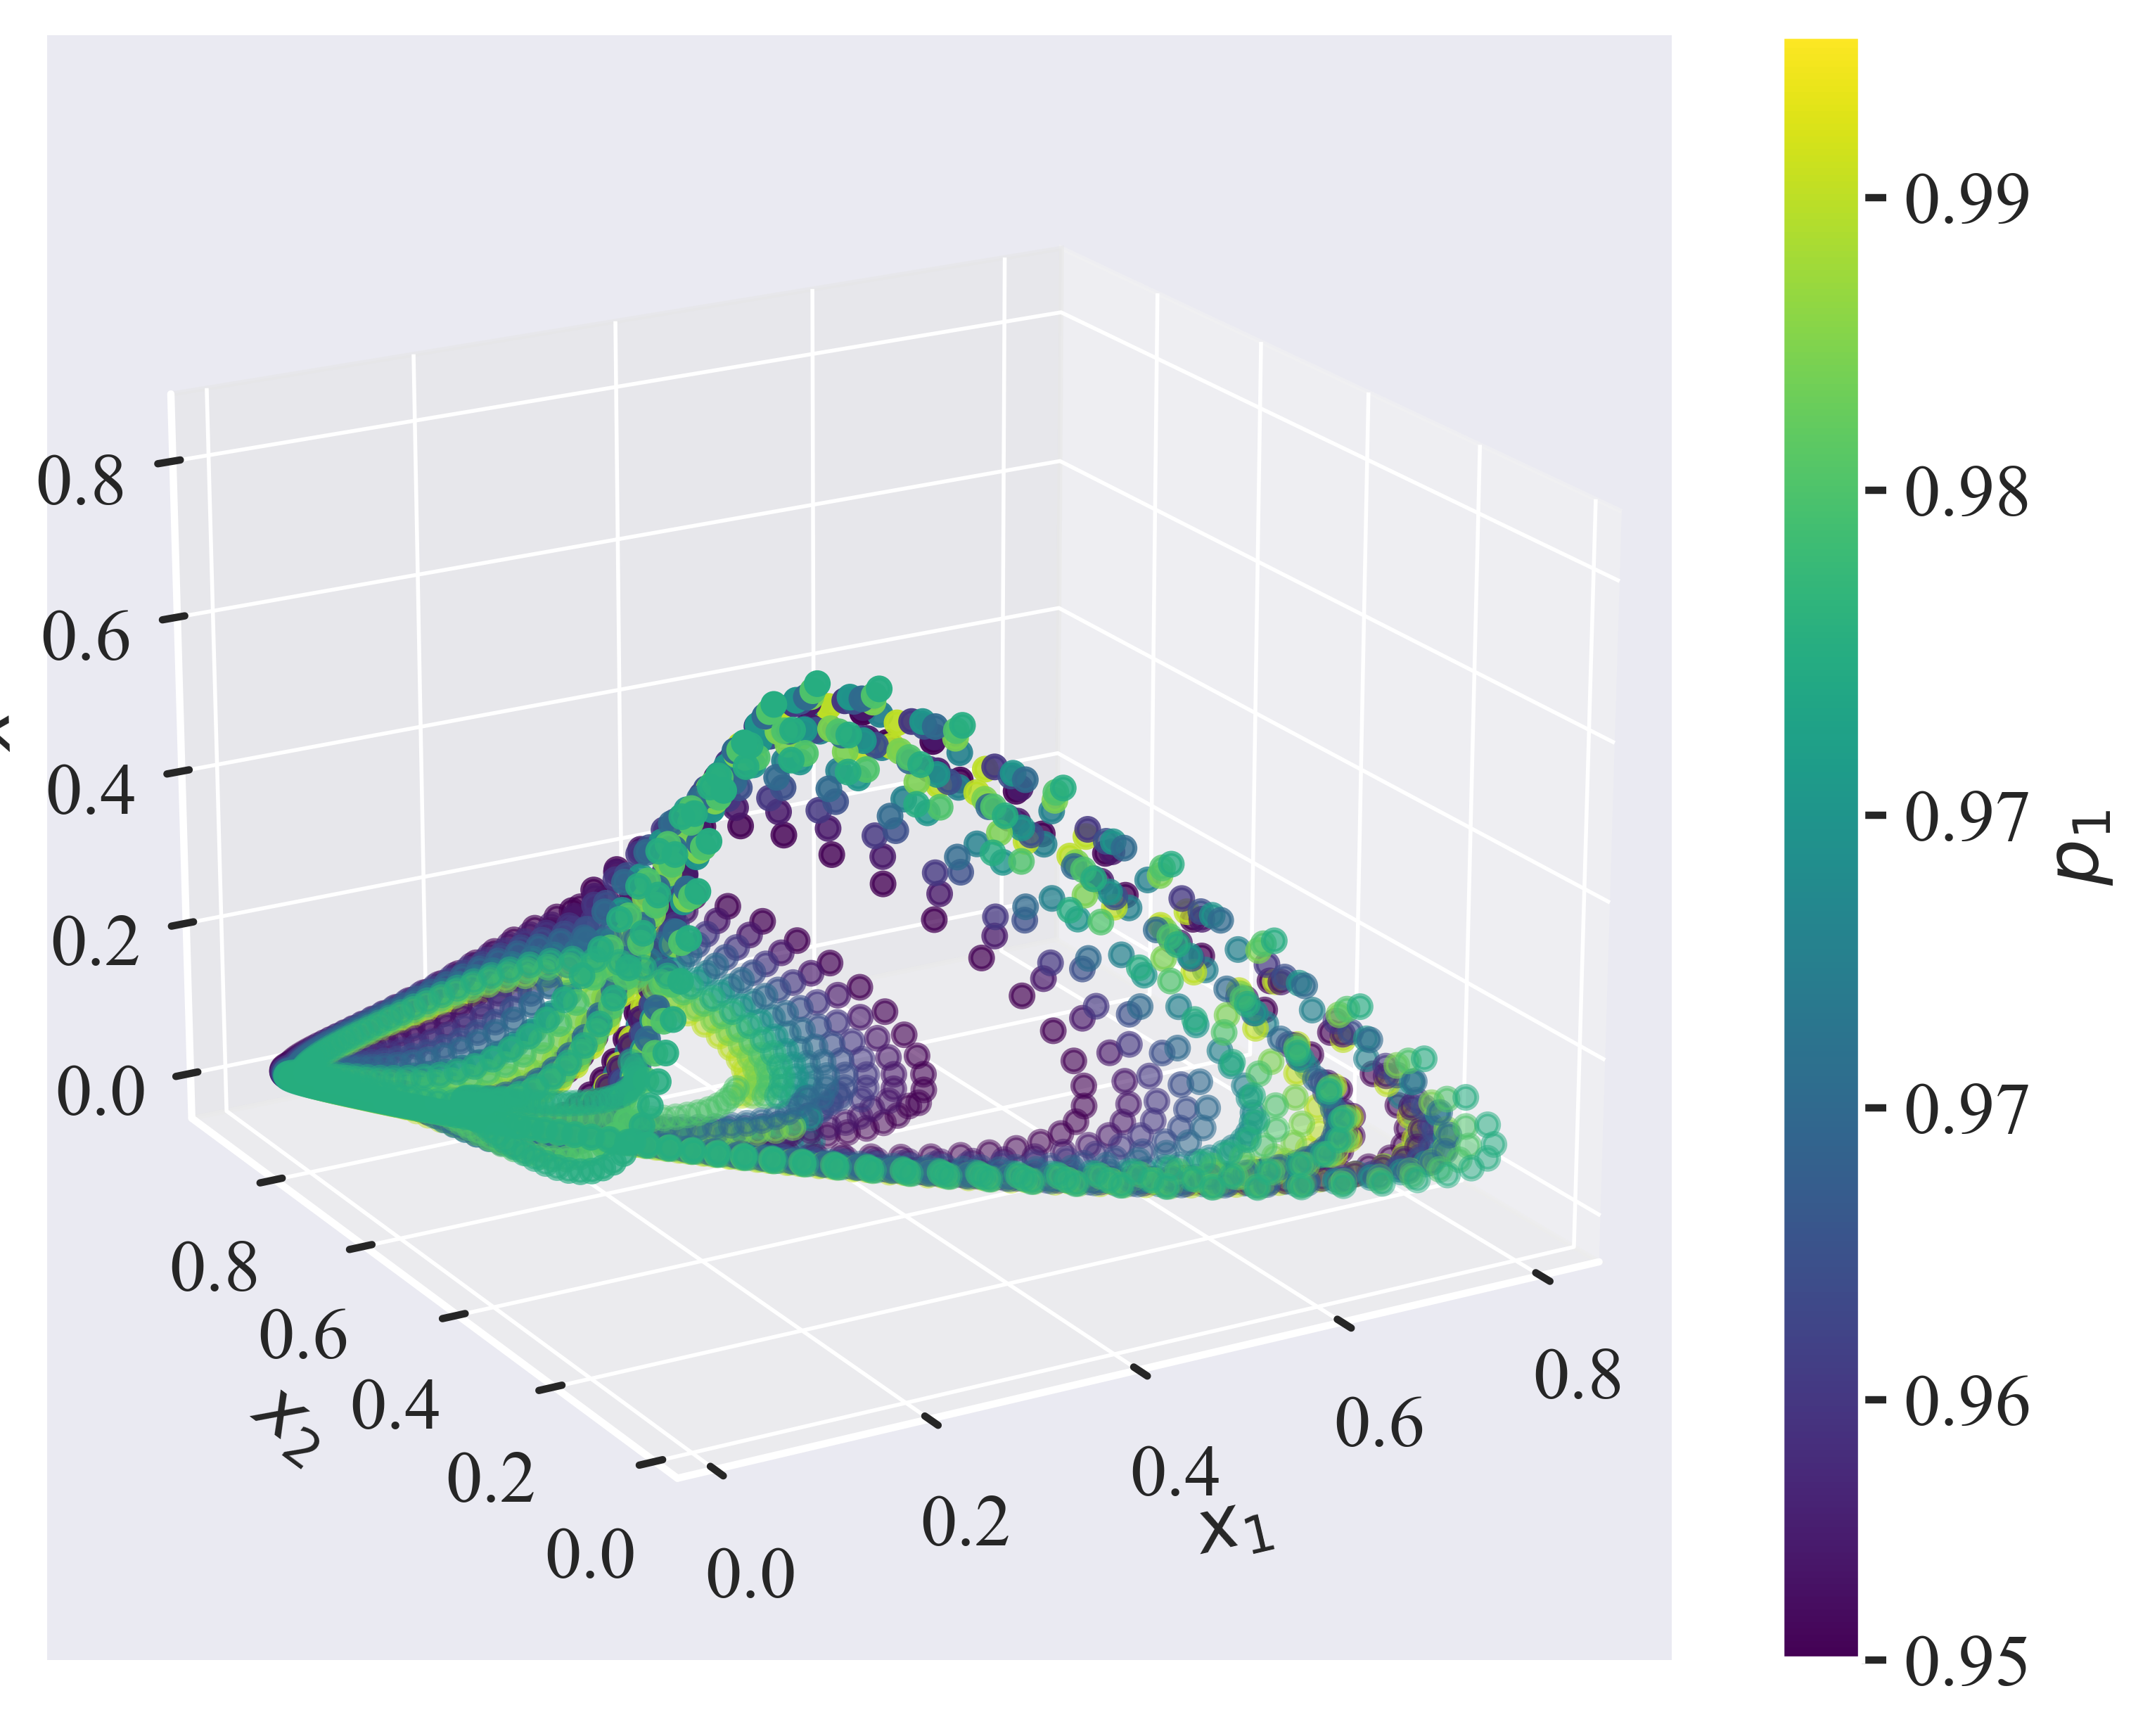
\includegraphics[width=0.7\textwidth]{figures/mcm_second_pdouble.png}
%     \caption{Continuation of the period-doubled limit cycle in the parameter $p_1$. The colors indicate the the flow of time
%     from dark to light.}
%     \label{fig:mcm_period_doubled_branch_2}
% \end{figure}
For instance, the third period-doubling bifurcation occurs at
\begin{align*}
    \textbf{Bifurcation type} & : \text{period doubling} \\
    \textbf{Label} &: \text{PD3} \\
    \textbf{Parameter} & : p_1 \\
    \textbf{Critical value} & : 0.949 \\
    \textbf{Floquet multipliers} & : -1.00, 0, 1.00 \\
    \mathbf{x}  & = (0.47, 0.19, 0.09) \\
    \textbf{Period} & : 130.3 \\
\end{align*}
However, this result must be taken with a grain of salt, as the remaining branch this bifurcation is unstable and seems
to rejoin the original limit cycle stemming from the Hopf bifurcation for $p_1 > 0.949$. 

As an alternative, we can predict the parameter values at which we expect period-doublings 
to occur using Feigenbaum's law (Equation 7.14, Seydel)
\begin{equation}
    \lim_{n \to \infty} \frac{p_{n+1} - p_n}{p_{n} - p_{n-1}} = 0.21416 \dots,
\label{eq:feigenbaum}
\end{equation}
This gives the following predictions for the period-doubling bifurcations in Table \ref{tab:period_doubling_predictions}.

\subsection{Route to chaos}
In order to determine whether a system exhibits chaos, we (numerically) calculate the Lyapunov exponents of the system.
We use the above predicted values for the period-doubling bifurcations as well as the point \textbf{PD3} as an initial condition.
Then we iteratively integrate the system over a large time-span ($t_{\textrm{end}} = 100$) with small timestep ($dt = 0.001$) and 
calculate the Lyapunov exponents at each iteration. The Lyapunov exponents are then averaged over time to obtain the approximate Lyapunov spectrum.
\footnote{this algorithm is adapted from 
\href[page=214]{http://ndl.ethernet.edu.et/bitstream/123456789/12518/1/80pdf.pdf}{CHAOS: An Introduction to Dynamical Systems} 
by Kathleen Alligood, section 5.2 "Numerical Calculation of Lyapunov Exponents", p.199 (214 in pdf).}
\begin{table}[H]
    \centering
    \begin{tabular}{|c|c|c|}
        \hline
        Period doubling & $p_1$ & Lyapunov spectrum \\
        \hline
        PD1 & $\mathbf{0.923}$ & 0.00, -0.04, -0.50 \\
        PD2 & $\mathbf{0.944}$ & 0.01, -0.06, -0.51 \\
        PD3 & 0.949 & 0.02, -0.06, -0.52 \\
        PD4 & 0.950 & 0.02, -0.06, -0.52 \\
        PD5 & 0.950 & 0.02, -0.06, -0.52 \\
        PD6 & 0.950 & 0.02, -0.06, -0.52 \\
        \hline
    \end{tabular}
    \caption{Predicted period doubling bifurcations using Feigenbaum's law and corresponding approximated Lyapunov exponents.
    \textbf{PD1} and \textbf{PD2} are taken from the continuation of the limit cycles, while the rest are predicted using
    the recurrence relation in Equation \ref{eq:feigenbaum}.}
    \label{tab:period_doubling_predictions}
\end{table}
We observe that one Lyapunov exponent is positive for values of $p_1 > 0.944$. This indicates that the system is chaotic for these values of $p_1$.

\subsection{Conclusion}
In the above treatment of the MCM system we 
\begin{enumerate}
    \item Found the stationary points of the system and continued the stable ones in the parameter $p_1$;
    \item Found a Hopf-bifurcation at $p_1 \approx 0.71$ and calculated the first limit cycle using the shooting method;
    \item Continued the limit cycle in the parameter $p_1$ and calculated the stability of the limit cycles;
    \item Found the first, second and third period-doubling bifurcations at $p_1 \approx 0.923$, $p_1 \approx 0.944$ and $p_1 \approx 0.949$, respectively;
    \item Verified the period-doubling bifurcations using Feigenbaum's law and calculated the Lyapunov exponents of the system;
    \item Determined that the system exhibits chaos for $p_1 > 0.949$.
\end{enumerate}
